%--------------------------------------
%VERSIÓN ANTIGUA. No la quiero eliminar porque me da tristeza.
\section{Sobre simetrías en las entradas de los polinomios de Legendre discretos (versión antigua)}
\label{section: sobre simetrias en las entradas de los poliomios discretos de Legendre (versión antigua)}

Puesto que planeamos implementar computacionalmente
las bases de Legendre discretas, es de utilidad 
buscar simetrías en las entradas de los vectores que las 
componen, pues esto puede reducir significativamente
el número de operaciones requeridas para el cálculo 
de bases de este tipo.
Ya los valores calculados
en la subsección 
\ref{formulas explicitas para Ln con n de 2 hasta 6}
sugieren 
la existencia de tales simetrías en las entradas 
del vector $\cali{L}^{n,k} \in \IR^{n}$.


\begin{figure}[H] \label{fig: simetrias entradas Legendre}
\centering\captionsetup{format = hang}
	\begin{measuredfigure}
		\includegraphics[scale=1.7]{simetrias_Legendre} 
		\caption{Parece ser que, en el vector,
		 $\cali{L}^{n,k} = \left( \cali{L}^{n,k}_{m} \right)_{m=0}^{n-1}$,
		las entradas a la derecha son iguales a las de la izquierda,
		con un cambio de signo que depende del
		grado $k$ del vector discreto de Legendre.}
		\label{fig: simetrias entradas Legendre}
 	\end{measuredfigure} 
 \end{figure}

A pesar de que, a estas alturas, ya contamos
con expresiones para los vectores $\cali{L}^{n,k}$
(para cualesquiera $n \in \IN$ y $0 \leq k \leq n-1$,
c.f. teorema \ref{teo: expresión analítica de BON de Legendre}),
no será usando estas que podremos demostrar que, en efecto,
se tienen las simetrías sugeridas en la figura
~\ref{fig: simetrias entradas Legendre}.
Conviene
usar una de las múltiples definiciones iniciales
que dimos para la base $\cali{L}^{n}$, a saber, una
que involucre discretizaciones puntuales de polinomios 
que de lugar a vectores $v_{k}$ que ya presenten 
este tipo de simetrías; por lo demostrado en secciones anteriores,
no perdemos generalidad al hacer esto. 


\begin{figure}[H]
\centering\captionsetup{format = hang}
	\begin{measuredfigure}
		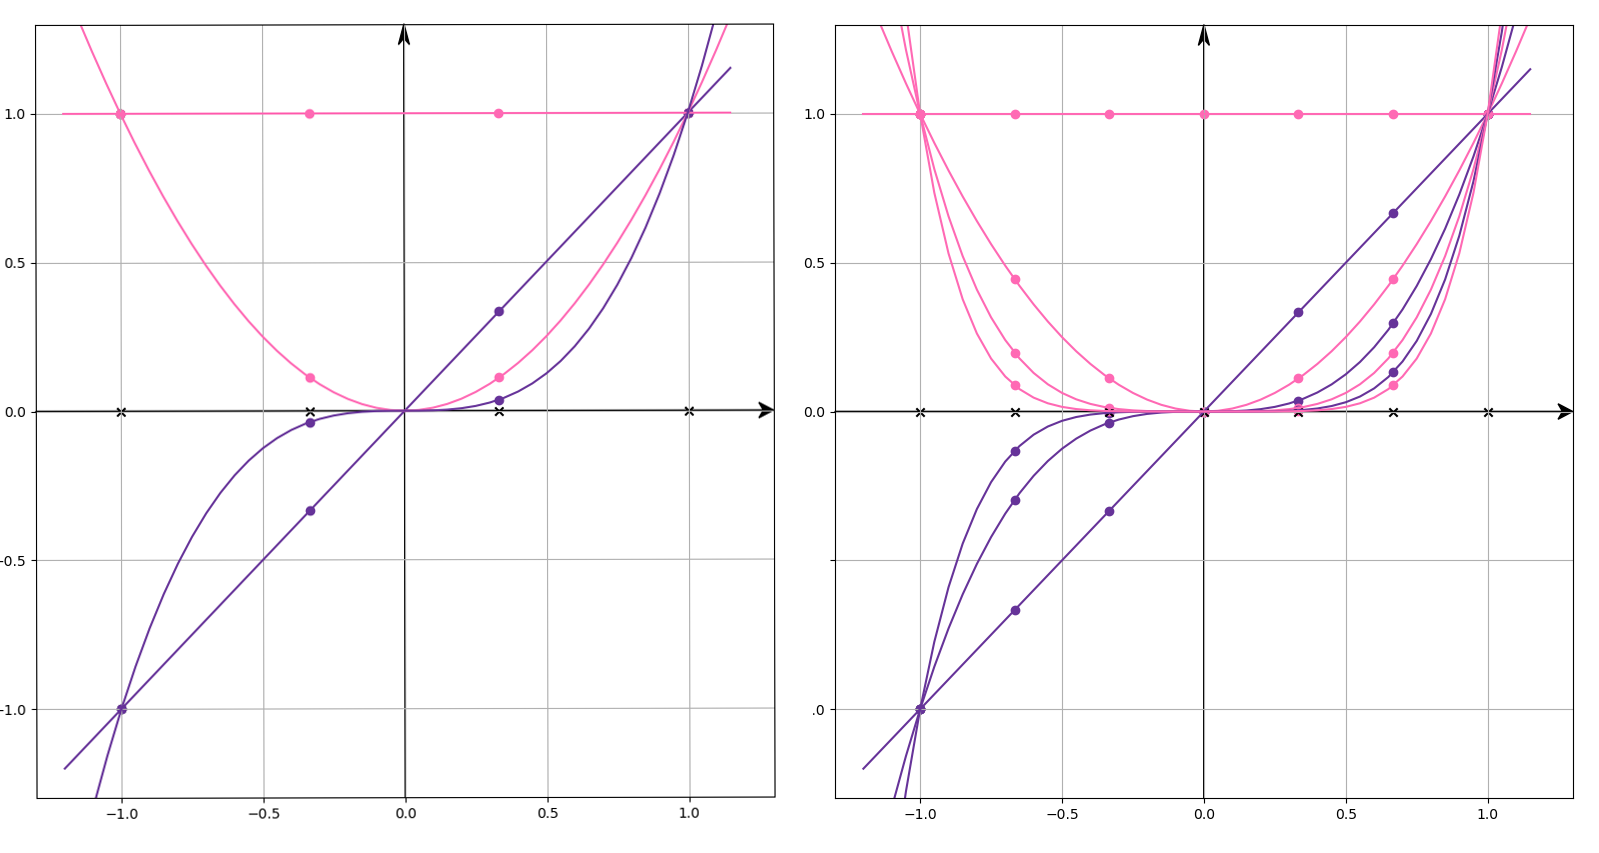
\includegraphics[scale=1]{10Dic_1} 
		\caption{En la figura se ilustran los polinomios y las
		mallas uniformes que escogeremos cuando las dimensiones sean
		$n=4$ (una dimensión par) y $n=7$ (una dimensión impar). Observe que
		las discretizaciones obtenidas con estas elecciones presentan
		las simetrías descritas en la figura 
		\ref{fig: simetrias entradas Legendre}.}
 	\end{measuredfigure}
 \end{figure}


Antes de enunciar los resultados 
principales de esta subsección, 
establecemos un lema que
engloba un argumento
central para todo lo que sigue.

\begin{lema}
\label{lema: lema para simetrias}
Sea $N \in \IN$. Sean $a_{m}$, con $0 \leq m \leq N$,
números reales. Sea la función de $N$ variables
\begin{equation}
\label{eq0: 9Dic}
f(x_{0}, \ldots , x_{N})= \suma{m=0}{N-1}{(a_{m}-x_{m})^{2}}
+ (a_{N}-x_{N})^{2} + \suma{m=0}{N-1}{(a_{m}+x_{m})^{2}}.
\end{equation}
La función $f$ tiene un mínimo en el punto
$(x_{0}, \ldots , x_{N})$, donde
$x_{m}=0$ para toda $0 \leq m \leq N-1$ y $x_{N}=a_{N}$.
\end{lema}
\noindent
\textbf{Demostración.}
Observando la distribución de las variables 
$x_{m}$ en la expresión \eqref{eq0: 9Dic}
que define a $f$,
podemos reescribir a la función $f$ a minimizar como sigue:
\begin{equation*}
f(x_{0}, \ldots , x_{N})= \suma{m=0}{N-1}{g_{m}(x_{m})}
+ h_{N}(x_{N}),
\end{equation*}
donde 

\begin{equation*}
g_{m}(x_{m}):= (a_{m}-x_{m})^{2}+ (a_{m}+x_{m})^{2},
\end{equation*}
y
\begin{equation*}
h_{N}(x_{N}):= (a_{N}-x_{N})^{2}.
\end{equation*}

Puesto que el minimizar una suma donde
cada sumando es positivo equivale a
minimizar cada uno de los sumandos,
en nuestro contexto tenemos que
hallar el punto $(x_{0}, \ldots , x_{N}) \in \IR^{N+1}$
que minimiza
a la función $f$ definida en 
\eqref{eq0: 9Dic} se obtiene al hallar,

\begin{itemize}
\item el punto $x_{N} \in \IR$ que minimiza a $h_{N}(x_{N})$, y
\item para toda $0 \leq m \leq N-1$, el punto $x_{m} \in \IR$
que minimiza a $g_{m}(x_{m})$.
\end{itemize} 

Calculando derivadas e igualando a cero, concluimos que
el mínimo de $f$ se alcanza cuando
\begin{equation}
x_{N}= a_{N}
\end{equation}
y
\begin{equation}
\forall \hspace{0.1cm} 0 \leq m \leq N-1 : \hspace{0.2cm}
x_{m}=0.
\end{equation}
\QEDB
\vspace{0.2cm}

\begin{prop}
\label{prop: para las simetrias en dimensiones impares}
\textbf{(Para dimensiones impares)}
Sea $n \in \IN$ impar, digamos,
$n=2N+1$, con $N \geq 1$. 
Sea $\cali{P}$ la malla
uniforme de $n$ puntos con puntos extremos $-1$ y $1$.
Para toda $0 \leq k \leq n-1$, sean
las potencias básicas $f_{k}(t)=t^{k}$ y los vectores
\begin{equation}
\label{eq4: 10Dic}
w_{k}=(w_{k,m})_{m=0}^{n-1} := \Omega_{n, \cali{P}}(f_{k}),
\end{equation}
donde $\Omega$ es el operador definido en 
\ref{def: operador de discretizacion puntual}, 
y $W_{n,k} \subseteq \IR^{n}$ 
el espacio definido en \ref{espacios Wi}.
Sean los subconjuntos de $\IR^{n}$
\begin{equation}
\label{eq0: 5Dic}
S_{+}:= \{ x=(x_{m})_{m=0}^{n-1}| \hspace{0.2cm} \forall  
\hspace{0.1cm}
0 \leq m \leq N-1 : \hspace{0.2cm} x_{m}= x_{2N-m}\}
\end{equation}
y

\begin{equation}
\label{eq1: 5Dic}
S_{-}:= \{ x=(x_{m})_{m=0}^{n-1}| \hspace{0.2cm} \forall  
\hspace{0.1cm}
0 \leq m \leq N-1 : \hspace{0.2cm} x_{m}= -x_{2N-m}\}
\end{equation}
Para toda $1 \leq k \leq n-1$
se tiene que
\begin{itemize}
\item $w_{k}- \Pi_{W_{n,k-1}}(w_{k}) \in S_{+}$ si $k$ es par, y
\item $w_{k}- \Pi_{W_{n,k-1}}(w_{k}) \in S_{-}$ si $k$ es impar.
\end{itemize}
\end{prop}
\noindent
\textbf{Demostración.}
Por ser los subconjuntos
de $\IR^{n}$ $S_{+}$ y $S_{-}$ trivialmente
no vacíos, cerrados bajo sumas
y productos por escalares, son subespacios
vectoriales de $\IR^{n}$. 

Por las simetrías de las funciones polinomiales
$f_{k}$ respecto a la malla $\cali{P}$, es obvio que,
para toda $0 \leq k \leq N-1$,

\begin{equation}
\label{eq1: 10Dic}
w_{k} \in S_{+} \hspace{0.2cm} \text{ si }
k \hspace{0.2cm} \text{ es par, }
\end{equation}
y
\begin{equation}
\label{eq2: 10Dic}
w_{k} \in S_{-} \hspace{0.2cm} \text{ si }
k \hspace{0.2cm} \text{ es impar.}
\end{equation}
Procedamos, ahora sí, a demostrar
la proposición por inducción sobre $k$.
\begin{itemize}
\item \textbf{(Base de inducción)}. 
Empecemos con el primer grado impar;
sea $k=1$. 
Según \eqref{eq2: 10Dic},
$w_{1} \in S_{-}$; digamos que
\begin{equation}
\label{eq3: 9Dic}
w_{1}=(a_{0}, \ldots , a_{N-1}, a_{N}, -a_{N-1}, \ldots , -a_{0} ).
\end{equation}
Puesto que $W_{n,0} \subseteq \IR^{n}$ consta 
de los polinomios discretos de
dimensión $n$ y grado cero (c.f. 
teorema \ref{cor: propiedades importantes de espacios Wi})
y $\Pi_{W_{n,0}}(w_{1}) \in W_{n,0}$, tenemos que
\begin{equation}
\label{eq4: 9Dic}
\Pi_{W_{n,0}}(w_{1})=(a, \ldots , a)
\end{equation}
para alguna $a \in \IR$.
Ahora bien, según el teorema
\ref{Teo:proyOrt} (en el que se da la propiedad definitoria de una proyección),
la constante $a$ es tal que
la norma (o, equivalentemente,
el cuadrado de la norma) del vector 
$w_{1}-\Pi_{W_{n,0}}(w_{1})$ es mínima; según 
\eqref{eq3: 9Dic} y \eqref{eq4: 9Dic}, tal norma
al cuadrado es 
\begin{equation}
\label{eq5: 9Dic}
|| w_{1}-\Pi_{W_{n,0}}(w_{1}) ||^{2}= 
\suma{m=0}{N-1}{(a_{m}-a)^{2}} + (a_{N}-a)^{2}
+ \suma{m=0}{N-1}{(a_{m}+a)^{2}};
\end{equation}
por el lema \ref{lema: lema para simetrias}, 
concluimos que el valor de $a$ que minimiza la expresión
\eqref{eq5: 9Dic}
(y que, por lo tanto, es el valor correcto), es
$a=0$.
Así, $\Pi_{W_{n,0}}(w_{1})$ es el vector cero, y
\[
w_{1}-\Pi_{W_{n,0}}(w_{1}) = w_{1} \in S_{-}.
\]
Sea ahora $k=2$, el primer grado par.
Según la proposición 
\ref{prop: los wk forman bases de los Wnk},
$W_{n,1} = span \{ w_{0}, w_{1}\}$;
puesto que, según 
\eqref{eq1: 10Dic} y \eqref{eq2: 10Dic}
se cumple
$\cali{L}^{n,0} \in S_{+}$ y 
$\cali{L}^{n,1} \in S_{-}$, tenemos que todo elemento de 
$W_{n,1}$ (en particular, la proyección $\Pi_{W_{n,1}}(w_{2})$)
puede expresarse como la suma de un elemento de $S_{+}$ y uno
de $S_{-}$; puesto que $w_{2} \in S_{+}$ y por ser la resta
de dos elementos de $S_{+}$ uno de este mismo espacio, inferimos que

\[
w_{2}-\Pi_{W_{n,1}}(w_{2})= \alpha - \beta,
\]
donde
$\alpha= S_{+}$ y $\beta \in S_{-}$.
Digamos que 

\begin{equation}
\label{eq2: 10Di}
\alpha = (a_{0}, \ldots , a_{N-1}, a_{N}, a_{N-1}, \ldots , a_{0})
\end{equation}
y 

\begin{equation}
\label{eq3: 10Di}
\beta = (b_{0}, \ldots , b_{N-1}, b_{N}, -b_{N-1}, \ldots , -b_{0}).
\end{equation}

Puesto que el cuadrado de la norma de 
$w_{2}-\Pi_{W_{n,1}}(w_{2})$ es mínimo, las entradas
$b_{m}$ del vector dado en 
\eqref{eq3: 10Di} son tales que la expresión
\begin{equation}
\label{eq6: 9Dic}
|| w_{2}-\Pi_{W_{n,1}}(w_{2}) ||^{2}= 
\suma{m=0}{N-1}{(a_{m}-b_{m})^{2}} + (a_{N}-b_{N})^{2}
+ \suma{m=0}{N-1}{(a_{m}+b_{m})^{2}}
\end{equation}
es mínima; según el lema 
\ref{lema: lema para simetrias}, esto implica que,
para toda $0 \leq m \leq  N-1$,
se tenga $b_{m}=0$.
Así, 
\begin{align*}
w_{2}-\Pi_{W_{n,1}}(w_{2}) =  \alpha - \beta
=  & (a_{0}, \ldots , a_{N-1}, a_{N}, a_{N-1}, \ldots , a_{0})-
(0, \ldots , 0, b_{N}, 0, \ldots ,0 ) \\
= & (a_{0}, \ldots , a_{N-1}, a_{N}-b_{N}, a_{N-1}, \ldots , a_{0}) \in S_{+}.
\end{align*}

\item \textbf{(Paso inductivo)}
Supongamos el resultado cierto para todo grado menor a $k$,
con $2 \leq k \leq n-1$.
Supongamos primero que $k$ es impar. Puesto que,
según la proposición 
\ref{prop: los wk forman bases de los Wnk},
$W_{n,k-1}= span \{ w_{K}: \hspace{0.2cm}
0 \leq K \leq k-1 \}$; además,
según \eqref{eq1: 10Dic} y \eqref{eq2: 10Dic},
tales vectores $w_{K}$ son
o bien elementos de $S_{+}$
o bien de $S_{-}$, tenemos que $\Pi_{W_{n,k-1}}(w_{k}) \in W_{n,k-1}$
puede expresarse como la suma de un elemento de $S_{+}$
y uno de $S_{-}$;
digamos que
\[
\Pi_{W_{n,k-1}}(w_{k}) = \gamma + \delta,
\]
con 
\begin{equation}
\label{eq: gamma}
\gamma = (c_{0}, \ldots , c_{N-1}, c_{N}, c_{N-1}, \ldots , c_{0}) \in S_{+}
\end{equation}
y 
$\delta \in S_{-}$.

Así, 
\[
w_{k} - \Pi_{W_{n,k-1}}(w_{k}) = w_{k} - (\gamma + \delta) = \epsilon - \gamma,
\]
donde $\epsilon := w_{k}-\delta$.
Como tanto $w_{k}$ como $\delta$ son elementos de $S_{-}$, 
tenemos también que
$\epsilon \in S_{-}$. Pongamos pues
\begin{equation}
\label{eq: epsilon}
\epsilon = (e_{0}, \ldots , e_{N-1}, e_{N}, -e_{N-1}, \ldots , -e_{0}) \in S_{-}.
\end{equation}
Usando el que $w_{k}-\Pi_{W_{n,k-1}}(w_{k})= \epsilon - \gamma$
y las expresiones \eqref{eq: gamma} y \eqref{eq: epsilon}
calculamos que 

\begin{equation}
\label{eq7: 9Dic}
|| w_{k}-\Pi_{W_{n,k-1}}(w_{k}) ||^{2}= 
\suma{m=0}{N-1}{(e_{m}-c_{m})^{2}} + (e_{N}-c_{N})^{2}
+ \suma{m=0}{N-1}{(e_{m}+c_{m})^{2}};
\end{equation}
puesto que $\Pi_{W_{n,k-1}}(w_{k})$ es el elemento
de $W_{n,k-1}$ que está más cerca
(en términos de la distancia euclidea) de $w_{k}$,
las entradas
$c_{m}$ de $\gamma$ son exactamente
los números reales que minimizan la expresión
\eqref{eq7: 9Dic}; esto, según el lema
\eqref{lema: lema para simetrias}, implica la igualdad 
a cero de todo $c_{m}$ con $0 \leq m \leq N-1$.
Concluimos así que 
\begin{align*}
w_{k}-\Pi_{W_{n,k-1}}(w_{k}) =  \epsilon - \gamma
=  & (e_{0}, \ldots , e_{N-1}, e_{N}, -e_{N-1}, \ldots , -e_{0})-
(0, \ldots , 0, c_{N}, 0, \ldots ,0 ) \\
= & (e_{0}, \ldots , e_{N-1}, e_{N}-c_{N}, -e_{N-1}, \ldots , -e_{0}) \in S_{-}.
\end{align*}

De un argumento análogo se sigue que, 
si $k$ era par, entonces
$w_{k}-\Pi_{W_{n,k-1}}(w_{k}) \in S_{+}$.
\end{itemize}
\null\nobreak\hfill\ensuremath{\square} %final dem
\vspace{0.2cm}

Las simetrías esperadas en las entradas de los vectores
de $\cali{L}^{n}$, cuando $n$ (la dimensión)
es un entero impar, se desprenden inmediatamente de
la proposición 
\ref{prop: para las simetrias en dimensiones impares}.

\begin{teo}
\label{prop: simetrias en dimensiones impares}
\textbf{(Para dimensiones impares)}. Sea $n \in \IN$ impar, digamos,
$n=2N+1$, con $N \geq 1$. Sea $0 \leq k \leq n-1$ y
considere al vector $\cali{L}^{n,k}=(\cali{L}^{n,k}_{m})_{m=0}^{n-1}$
como se ha definido en \eqref{def: base de Legendre discreta}.
Para toda $0 \leq m \leq N-1$ se tiene que
\begin{itemize}
\item $\cali{L}^{n,k}_{m} = \cali{L}^{n,k}_{2N-m}$ si $k$ es par y
\item $\cali{L}^{n,k}_{m} = -\cali{L}^{n,k}_{2N-m}$ si $k$ es impar.
\end{itemize}


\begin{figure}[H]
\centering\captionsetup{format = hang}
	\begin{measuredfigure}
		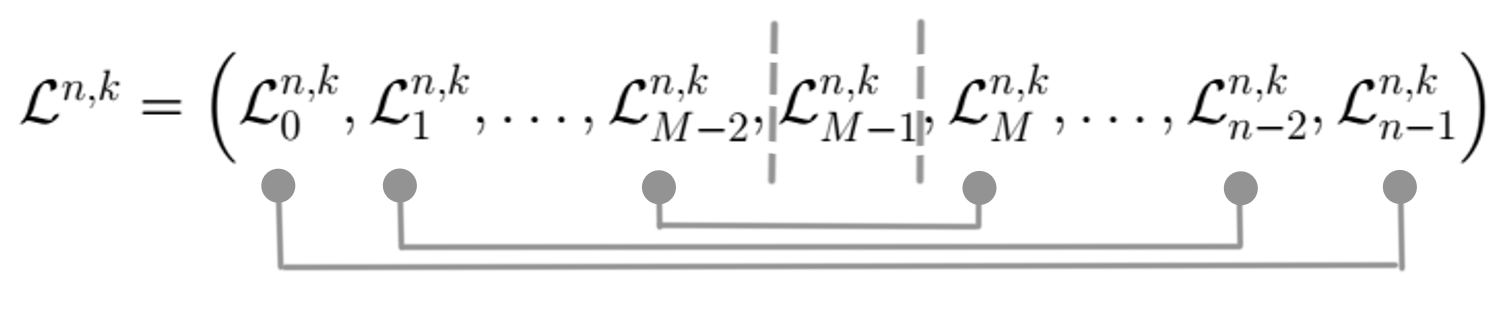
\includegraphics[scale=1]{simetria1} 
		\caption{Fijadas una dimensión impar $n=2N+1$ 
		y un grado $0 \leq k \leq n-1$,
		en esta proposición se da una relación simple entre las parejas 
		de entradas de $\cali{L}^{n,m}$ con índices $m$ y $2N-m$ 
		(donde los índices $0 \leq m \leq N-1$ son los de las primeras
		$N$ entradas).}
 	\end{measuredfigure}
 \end{figure}
\end{teo}
\noindent
\textbf{Demostración.}
Según la teoría desarrollada en la subsección
\ref{Generalización que involucra a la discretización Omega n},
una forma de construir a 
la base $\cali{L}^{n}$ consiste en 
considerar a las $n$ funciones polinomiales
\[
f_{k}(t)= t^{k}, \hspace{0.2cm} 0 \leq k\leq n-1,
\]
discretizar a estas en la malla uniforme de $n$ puntos
cuyos puntos extremos son $-1$ y $1$, para así obtener
vectores $w_{k}=(w_{k,m})_{m=0}^{n-1}$; como se 
demuestra en tal subsección, se tiene que
\begin{equation} 
\label{eq2: 9Dic}
\cali{L}^{n,0}= 
\left( \frac{1}{\sqrt{n}}, \ldots , \frac{1}{\sqrt{n}} \right),
\end{equation}
y, para toda $1 \leq k \leq n-1$,
\begin{equation} 
\label{eq1: 9Dic}
\cali{L}^{n,k}= 
\frac{w_{k}- \Pi_{W_{n,k-1}}(w_{k})}{|| w_{k}- \Pi_{W_{n,k-1}}(w_{k}) ||},
\end{equation}
donde los espacios $W_{n,k-1}$ son como 
se definieron en \eqref{espacios Wi}.


De la ecuación \eqref{eq2: 9Dic} se sigue de inmediato
la veracidad del teorema
para el grado $k=0$.

Sea ahora $1 \leq k \leq n-1$.
Considere a los subespacios $S_{+}$
y $S_{-}$ de $\IR^{n}$ como se definieron en 
\eqref{eq0: 5Dic} y \eqref{eq1: 5Dic}.
Según la proposición 
\ref{prop: para las simetrias en dimensiones impares}, 
el vector $w_{k}- \Pi_{W_{n,k-1}}(w_{k})$
es elemento de $S_{+}$ si $k$ es par y es elemento 
de $S_{-}$ si $k$ es impar; pero,
según \eqref{eq1: 9Dic},
los vectores $\cali{L}^{n,k}$ y 
$w_{k}- \Pi_{W_{n,k-1}(w_{k})}$
difieren sólo por la multiplicación
de un escalar; por ser
$S_{+}$ y $S_{-}$ ambos subespacios de $\IR^{n}$, 
concluimos de esto la pertenencia 
de $\cali{L}^{n,k}$ a $S_{+}$ siempre que $k$ sea par,
y a $S_{-}$ cuando $k$ sea impar.
\null\nobreak\hfill\ensuremath{\square} %final dem
\vspace{0.2cm}


Resultados análogos a los
\ref{prop: para las simetrias en dimensiones impares}
y 
\ref{prop: simetrias en dimensiones impares} se establecen
cuando la dimensión $n$ 
del espacio es par, pues en ambos resultados 
nunca se habló de la entrada central (a saber, $\cali{L}^{n, k}_{N}$),
sino que siempre se trató de establecer igualdades entre
entradas opuestas del vector $\cali{L}^{n,k}$
(que se obtienen reflejando respecto a la entrada central 
$\cali{L}^{n, k}_{N}$).
No damos pues el análogo a la proposición 
\ref{prop: para las simetrias en dimensiones impares} 
(que fue un resultado auxiliar para establecer la simetría buscada)
y establecemos, sin demostración, la contraparte del
teorema
\ref{prop: simetrias en dimensiones impares} 
para dimensiones pares.


\begin{teo}
\label{prop: simetrias en dimensiones pares}
\textbf{(Para dimensiones pares)}. Sea $n \in \IN$ par, digamos,
$n=2N$, con $N \geq 1$. Sea $0 \leq k \leq n-1$ y
considere al vector $\cali{L}^{n,k}=(\cali{L}^{n,k}_{m})_{m=0}^{n-1}$
como se ha definido en \eqref{def: base de Legendre discreta}.
Para toda $0 \leq m \leq N-1$ se tiene que
\begin{itemize}
\item $\cali{L}^{n,k}_{m} = \cali{L}^{n,k}_{2N-m-1}$ si $k$ es par y
\item $\cali{L}^{n,k}_{m} = -\cali{L}^{n,k}_{2N-m-1}$ si $k$ es impar.
\end{itemize}

\begin{figure}[H]
\centering\captionsetup{format = hang}
	\begin{measuredfigure}
		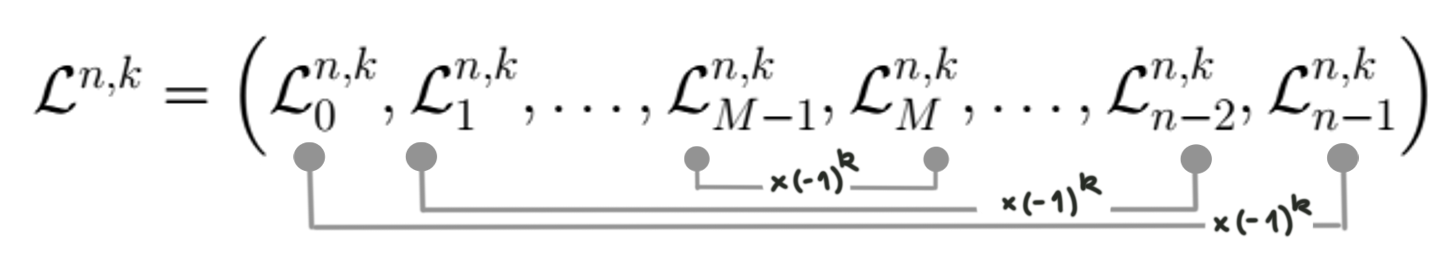
\includegraphics[scale=1]{simetria2} 
		\caption{Fijadas una dimensión par $n=2N$ 
		y un grado $0 \leq k \leq n-1$,
		en esta proposición se da una relación simple entre las parejas 
		de entradas de $\cali{L}^{n,m}$ con índices $m$ y $2N-m-1$ 
		(donde los índices $0 \leq m \leq N-1$ son los de las primeras
		$N$ entradas).}
 	\end{measuredfigure}
 \end{figure}
\end{teo}

Gracias a lo demostrado en esta sección, sabemos que,
fijada una dimensión $n$ y fijado un grado $0 \leq k \leq n-1$,
el cálculo de las $n$ entradas del vector $\cali{L}^{n,k}$
se reduce al cálculo de la mitad de estas, pues las otras pueden
deducirse de las primeras con un cambio de signo que está completamente
determinado por la paridad del grado $k$.


\begin{figure}[H]
\centering\captionsetup{format = hang}
	\begin{measuredfigure}
		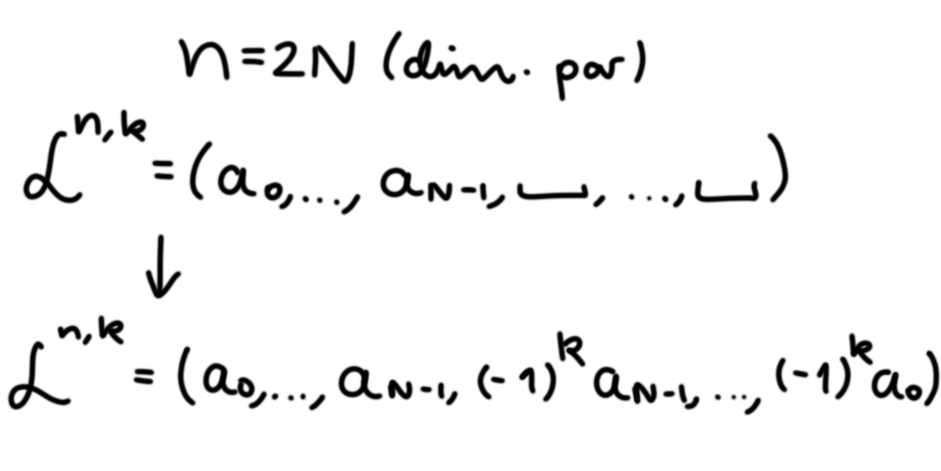
\includegraphics[scale=1]{10Dic_3} 
		\caption{\TODO{aaa}}
 	\end{measuredfigure}
 \end{figure}

Observe que, en el caso de dimensiones impares, no se dijo nada
sobre la entrada central de los vectores $\cali{L}^{n,k}$;
para finalizar esta sección, digamos para qué grados $k$
es seguro que tal entrada central sea cero.

\begin{teo}
\textbf{(para dimensiones impares)}.
Sea $n \in \IN$ impar, digamos,
$n=2N+1$, con $N \geq 1$. Sea $0 \leq k \leq n-1$ y
considere al vector $\cali{L}^{n,k}=(\cali{L}^{n,k}_{m})_{m=0}^{2N}$
como se ha definido en \eqref{def: base de Legendre discreta}.
Si $k$ es impar, entonces la entrada central del vector
$\cali{L}^{n,k}$ es cero, o sea, 
\[
\cali{L}^{n,k}_{N}=0.
\]
\end{teo}
\noindent
\textbf{Demostración.}
Según el teorema 
\ref{prop: simetrias en dimensiones impares}, 
$\cali{L}^{n,k} \in S_{-}$, 
donde $S_{-}$ se ha definido en \eqref{eq1: 5Dic},
o sea,
\begin{equation}
\label{eq2: 5Dic}
\forall \hspace{0.1cm}
0 \leq m \leq n-1: \hspace{0.2cm} \cali{L}^{n,k}_{m}= 
-\cali{L}^{n,k}_{2N-m}.
\end{equation}
Además, según el corolario
\ref{cor: Ln,k ortogonal a todo pol discreto de grado menor a k},
los vectores
$\cali{L}^{n,0}= \left( \frac{1}{\sqrt{n}},
\ldots , \frac{1}{\sqrt{n}} \right)$ y $\cali{L}^{n,k}$
son ortogonales, luego, 
\[
0= \langle \cali{L}^{n,0}, \cali{L}^{n,k} \rangle
=  \frac{1}{\sqrt{n}} \cdot \suma{m=0}{^{n-1}}{\cali{L}^{n,k}_{m}}
= \frac{1}{\sqrt{n}} \cdot \cali{L}^{n,k}_{N},
\]
dándose esta última igualdad por ocurrir
\eqref{eq2: 5Dic}. Concluimos así, como queríamos, que 
$\cali{L}^{n,k}_{N}=0$.
\null\nobreak\hfill\ensuremath{\square} %final dem
\vspace{0.2cm}
